
\documentclass{beamer}
% \setbeamertemplate{navigation symbols}{}
%\setbeamercolor{frametitle}{fg=black,bg=white}
%\setbeamercolor{title}{fg=black,bg=yellow!85!orange}
\usetheme{Boadilla}
\usepackage{makecell}
\usepackage{booktabs}
\usepackage{caption}
\usepackage{physics}
\usepackage{xcolor}
\usepackage{multirow}
\usepackage{bm}
\usepackage{ragged2e}
\apptocmd{\frame}{}{\justifying}{}

% \beamersetuncovermixins{\opaqueness<1>{25}}{\opaqueness<2->{15}}
\begin{document}
	\title[Bayesian Hierarchical Clustering]{Bayesian Hierarchical Clustering for CyTOF: A Research Proposal}
	\author{Mukai Wang}
	
	\begin{frame}
		\titlepage
	\end{frame}
	
	\begin{frame}
		\tableofcontents[hideallsubsections]
	\end{frame}

	\section{Hierarchical Clustering}
	\subsection{SPADE}
	
	\begin{frame}
		\tableofcontents
		[
		currentsection,
		currentsubsection,
		subsectionstyle=show/shaded/hide
		]
	\end{frame}
	
	\begin{frame}{SPADE Clustering}
		\begin{figure}[htbp]
			\centering
			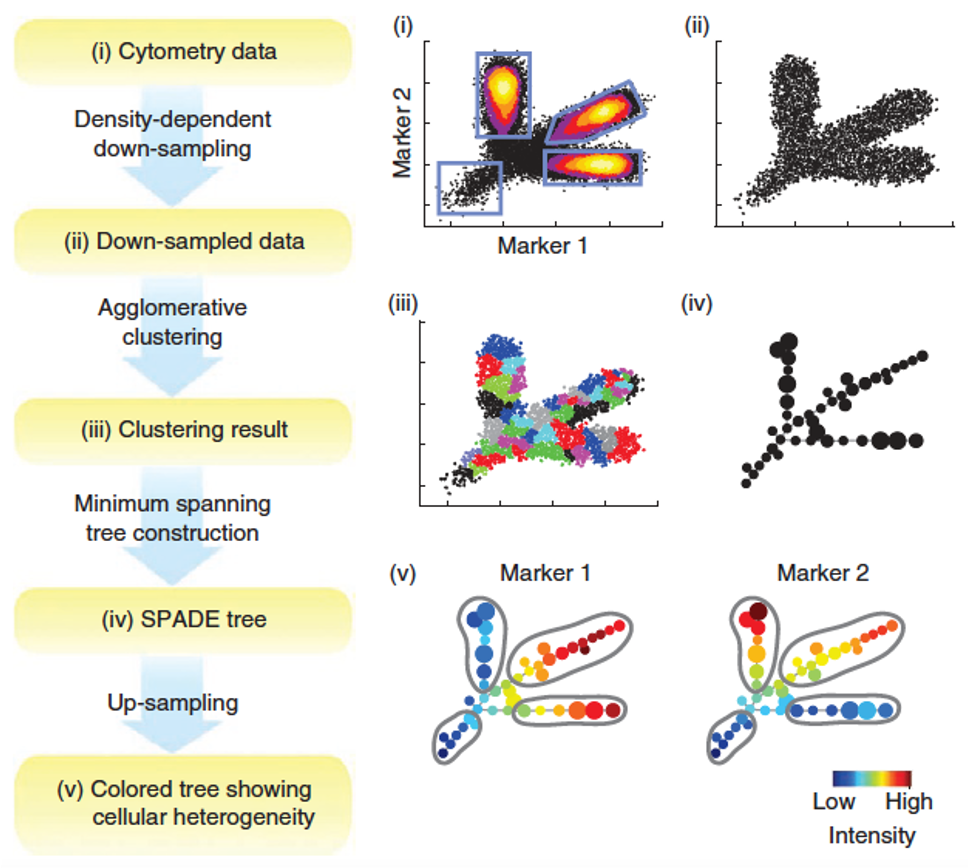
\includegraphics[scale=0.5]{SPADE.png}
			\caption*{Qiu etal \emph{Nature Biotechnology} 2011}
		\end{figure}
	\end{frame}
	
	\section{Bayesian Statistics}
		\begin{frame}
		\tableofcontents
		[
		currentsection,
		currentsubsection,
		subsectionstyle=show/shaded/hide
		]
	\end{frame}
	\section{Dirichlet Prior for Bayesian Clustering}
		\begin{frame}
		\tableofcontents
		[
		currentsection,
		currentsubsection,
		subsectionstyle=show/shaded/hide
		]
	\end{frame}
	\section{Dirichlet Diffusion Tree Prior for Bayesian Clustering}	
		\begin{frame}
		\tableofcontents
		[
		currentsection,
		currentsubsection,
		subsectionstyle=show/shaded/hide
		]
	\end{frame}
\end{document}